\documentclass[11pt]{myclass}
\usepackage[margin=1in]{geometry}
\usepackage{mathptmx}
\usepackage{color}
\usepackage{hyperref}
\usepackage{verbatim}
\usepackage{amssymb}
\usepackage{algorithm, algorithmic}


\newcommand{\breg}{\ensuremath{D_\phi}}
\newcommand{\sbreg}{\ensuremath{D_{s\phi}}}
\newcommand{\eps}{\varepsilon}

\title{CS 5350 Final Project Report}
\author{Vishay Vanjani, Alex Clemmer, \textit{Godzillasaurus Rex}}
%\date{} % Activate to display a given date or no date (if empty),
         % otherwise the current date is printed 

\begin{document}
\maketitle

\section{Architecture of your IE system}

Our system is a composite prediction system, with every slot predicted individually. Although we experimented with a number of different approaches, our final system used \textit{AutoSlog-TS} for 3 of the 6 slots, a decision we made mainly on the strength of the algorithm's results for \texttt{test set 1}. Slots that were not covered using AutoSlog-TS were either not tractable for the algorithm, or we found a better solution, using some performance measure. The slots not covered were \texttt{incident}, \texttt{weapons}, and \texttt{perp\_org}. \texttt{incident} prediction was handled with a custom pattern-matching system; \texttt{weapons} and \texttt{perp\_org} were handled by a weighted histogram lookup.

\subsection{Predicting the \texttt{Incident} Slot}

We manually created around 50 patterns, linking each to an \textit{incident type} (\textit{e.g.}, ``\texttt{attack}"). For each particular text, we scored each pattern, and output the incident type of the pattern that had the best score. Our default fallback was to simply output \texttt{attack}. The scoring of a pattern is a straightforward combination of the hand-annotated relevance of pattern and the frequency of pattern.

\subsection{Predicting Slots Using AutoSlog-TS (\texttt{Perp\_Ind}, \texttt{Targets}, and \texttt{Victim})}

We used AutoSlog-TS to automatically extract a lot of relevant patterns from the \texttt{dev} and \texttt{test1} sets, which we could then annotate as useful for a particular slot, or discard. We did this on a \textit{per-slot} basis, and initially, we had a parallel system for every slot except the \texttt{Incident} slot (which we already had a good predictor for) and the \texttt{Perp\_Org} slot. After manual review we found no relevant patterns for \texttt{weapons}.

The output of this system was 99 total patterns, which were then used at runtime to extract the context surrounding the set of probable possible answers. A summary of our this output is here (and you can see the extracted patterns in Appendix A \& B): \\

\begin{tabular}{| l | c | r |}
  \hline
  \textbf{Slot} & \textbf{Unique Patterns Extracted} & \textbf{Patterns after manual review} \\
  \hline
  \hline
  \texttt{Victims} & 1021 & 45 \\
  \hline
  \texttt{Targets} & 1169 & 21 \\
  \hline
  \texttt{Perp\_Indiv} & 521 & 33 \\
  \hline
  \texttt{Weapons} & 108 & 0 \\
  \hline
  \hline
  \textbf{Total} & \textbf{2819} & \textbf{99} \\
  \hline
\end{tabular}

\subsubsection{AutoSlog-TS Pipeline}

AutoSlog of course required a certain amount of scaffolding to work.

\begin{enumerate}

\item \textbf{Preprocessing:} Separate the header metacontent from the text, and things like that.

\item \textbf{Parsing and NP-chunking:} We parsed the main content of the page using the Stanford parser and used the parsed tree to build a NP chunked output.

\item \textbf{AutoSlog-TS:} We used regular expressions to look for heuristics in the chunked text and used the AutoSlog scoring mechanism to rank the extracted patterns.

\end{enumerate}

Note that our pattern ranking criteria were: $relevance-rate \cdot \log_2(frequency)$. A pictoral summary of the process is here: \\

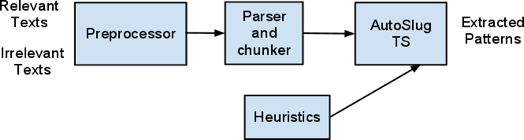
\includegraphics[scale=0.75]{workflow.png}

\subsubsection{Pattern Extraction in AutoSlog-TS}

We used a total of 13 heuristics for our system, 7 of these were for \texttt{Victim}, 4 were for \texttt{Target}, 2 were for \texttt{Perp\_Indiv} and 1 was for \texttt{Weapon}. There was one overlapping heuristic between \texttt{Victim} and \texttt{Target}. As we saw in the table in section 1.2, this resulted in a total of 99 unique patterns.

One particular challenge was that we had to modify the heuristics given in the paper[1] to suit our parser, first, because our it did not distinguish between active voice and passive voice, and second, because it did not identify syntactic roles (\textit{e.g.} subject, direct object, etc.) Of course, it is true that the dependency lists output by the parser could possibly be used to identify subjects and direct objects, but they were \textit{prima facie} not very accurate, so we decided not to use them.

\subsubsection{Pattern Matching in AutoSlog-TS}

This step occurs at runtime, after we've extracted patterns from the text. Our job at this point is basically to find patterns in a given text, rank the patterns that are most likely to contain correct predictions for a given slot, and then strip out the extraneous information we've extracted along with the embedded answer. The process is as follows:

\begin{enumerate}

\item \textbf{Preprocessing:} Splits the file into multiple texts and splits each text into meta text and main text. 

\item \textbf{Sentence-Splitting:} Splits the main text into different sentences using two patterns 1) dot followed by space or 2) dot followed by quotes.

\item \textbf{Pattern Matching:} Uses regular expressions to match the extracted patterns for victims, targets, and perpetrators in a given sentence. For our purposes, the forward patterns were the patters in which the relevant NP occured at the beginning (e.g ``\texttt{<NP> WAS\textbackslash s*[\textbackslash w]*\textbackslash s*MURDERED}"). In contrast, backward patterns are patterns in which the relevant NP occurs at the end (e.g. ``\texttt{MURDERED <NP>}” ). We looked for forward patterns first and then for backward patterns, if a forward pattern matched then the backward pattern containing the same verb is not considered. For example, if  ``\texttt{WAS\textbackslash s*[\textbackslash w]*\textbackslash s*MURDERED}" matched then we did not look for ``\texttt{MURDERED <NP>}".

\item \textbf{Parsing and NP Chunking:} If a sentence matches a particular pattern then we extract the relevant NP (i.e., for forward patterns we extract NP occurring just before the pattern and for backward patterns we extract the NP occurring after the pattern).

\end{enumerate}

A pictoral representation of this process is here:


\includegraphics[scale=0.75]{patt.png}

\subsubsection{Post Proessing in AutoSlog-TS}

This module’s goal was to filter through the list of NPs returned by previous step before choosing the correct answers for each slot. We wrote methods that performed the following tasks in order to complete this module. 

\begin{enumerate}

\item \textbf{Extracting Multiple Answers from an NP:} We found that in some cases the extracted NP contained multiple answers separated by “and“, “accompanied by”, etc. We chose to look for such words and split the NP appropriately.

\item \textbf{Removing Synonyms:} We had a hard coded list of synonyms for this task. 

\item \textbf{Overlapping Answers Removal:} We often found that some of our answers overlapped (e.g., Hector Oqueli and Oqueli). In these cases, we simply chose the largest of the two strings.

\item \textbf{Appositive Removal:} Our answers for the victim slot usually contained appositives like ``Obama, President of the United States". So we maintained a list of relevant appositives and removed these if they were a part of the NP.

\item \textbf{Flag List:} We maintain flag list for all 3 of the slots. Flag list marks NPs that should be removed from consideration. For example, a victim flag list contained these words like \textit{headquarters} and \textit{embassy}. If such an NP in the list was reported, we simply removed it.

\item \textbf{Redundant word List:} This is a list of unnecessary words like verbs, weekdays, and prepositions that may be found alongside the answer, but which destroy the correctness of our answers.

\item \textbf{One word List:} This is a list of words which on their own could not be answers to any of the slots. Examples include words like \textit{headquarters}, \textit{urban}, \textit{salvador}, and so on. These words were summarily removed from any answers.

\end{enumerate}

\subsection{Predicting the \texttt{Weapon} slot}






\section{External resources}

Our final project uses NLTK and the Stanford Parser. However, we also at various points in the project used the Berkeley Parser, the Collins Parser, and the Stanford NER tagger, and both the lexicalized and normal Stanford PCFG parsers. NLTK was used for sentence and word tokenization, in addition to pos tagging and chunking.

\section{Contribution of each team member}

For a given slot, we ended up deploying the system that was most effective on the \texttt{test1} set. Although we performed many experiments, the \texttt{Victim}, \texttt{Perp\_Indiv}, and \texttt{Target} slots all ended up having an AutoSlog-TS backend, which was implemented almost entirely by \textbf{Vishay}. He was responsible for the pre- and post-processing of the AutoSlog system, as well as almost all of the internals. Finally, he implemented the initial \texttt{Incident} predictor, which was responsible largely for our score in the dry run.

The remaining slots were \texttt{Perp\_Org} and \texttt{Weapon}, both implemented by \textbf{Alex}. Additionally, Alex was responsible for integrating all the systems together, testing all the systems, and tuning the output. Further, Alex spent much of his time trying to produce viable alternatives to AutoSlog-TS, and although you won't see them in the final system, you can still see the code in the repository (especially if you sift through the commits in the .git file). Outlines of the approaches in the presentation slides, and, to a lesser extent, in the ``originality" section.

\section{Emphasis / Originality}

We started our project thinking that extracting the relevant patterns will be the most important part of the project, and because we did not want any bias in selecting of Patterns, we decided to go with the AutoSlug- TS approach. However we later found that the Post Processing phase was as important as the Pattern Selection phase. We were extracting a lot of irrelevant NPs and the few relevant NPs that we were extracting were filled with redundant words. Our most original module was the Post processor ( and Weapns ???? ) because we tried a lot of unique things in that module. However it was also the least robust part of our project.

\section{Performance results and “glass box” analysis}

\section{Surprise Factor}

\begin{enumerate}

\item Among 4 different parsers, we could barely get coherent output. To chunk NPs it was much more effective to word-tokenize, and then use NLTK's builtin NP chunker to find NPs.

\item We had not anticipated that the post processing module to be as complicated as it was. It was really difficult to sift through all the NPs extracted and get the correct answers.

\item Simple techniques worked better. Most people who had mined their answers from \texttt{dev} set did really well, even for general slots like \texttt{Victim}, \texttt{Target}, and \texttt{Perpet\_Indiv}.

\end{enumerate}

\section{Successes, regrets, and lessons learned}

Our success is straightforward: we were best-in-class on the \texttt{test1} set. This is undisputable. We also tried out a huge number of techniques and technologies, and were even successful in producing competetive results in other approaches that we tried.

That said, our results on the \texttt{test2} set were very bad, mainly because our post processing step was manually developed using only the \texttt{test2} data. This caused massive overfitting, and in retrospect, there are a number of different ways this could have been avoided:

\begin{enumerate}

\item Building the system on the \texttt{dev} set alone, and using the test set \textit{only} for tuning.
\item Building an ML-based post processor.
\item Using an NER tagger plus a dictionary (for nameless victimsm \textit{e.g.}, people, child, wife, etc.) to validate the answers for the victim slot.

\end{enumerate}


This is a big lesson not really because we didn't know about overfitting before (we did), but because it makes the lesson of overfitting \textit{very} concrete: avoid anything that even \textit{looks} like overfitting.





\end{document}